%capitulo08
\label{cap:schedule}
\noindent 

This section presents the schedule of activities for the development of this doctoral research project, starting in April of 2016 and ending in March 2020, totalling a period of 48 months. The dependence between the steps can lead, at some point, to changes in the schedule, and its restructuring is necessary. The activities of the nearest steps have a more detail level than those of the later steps, which are in a higher level of abstraction, because, as discussed in Section~\ref{cap:methodology}, with each step start, there is a planning in which discussed and listed the next activities and artefacts produced.
The focus of research from the present moment will be on the choice of approach to the research problems described in  Section~\ref{cap:researchproblems}.
Table~\ref{tab:schedule1} presents the planning of the academic training activities and the planning of the research activities.

\begin{table*}[htbp]
	\centering
	\caption{Schedule of activities.}
    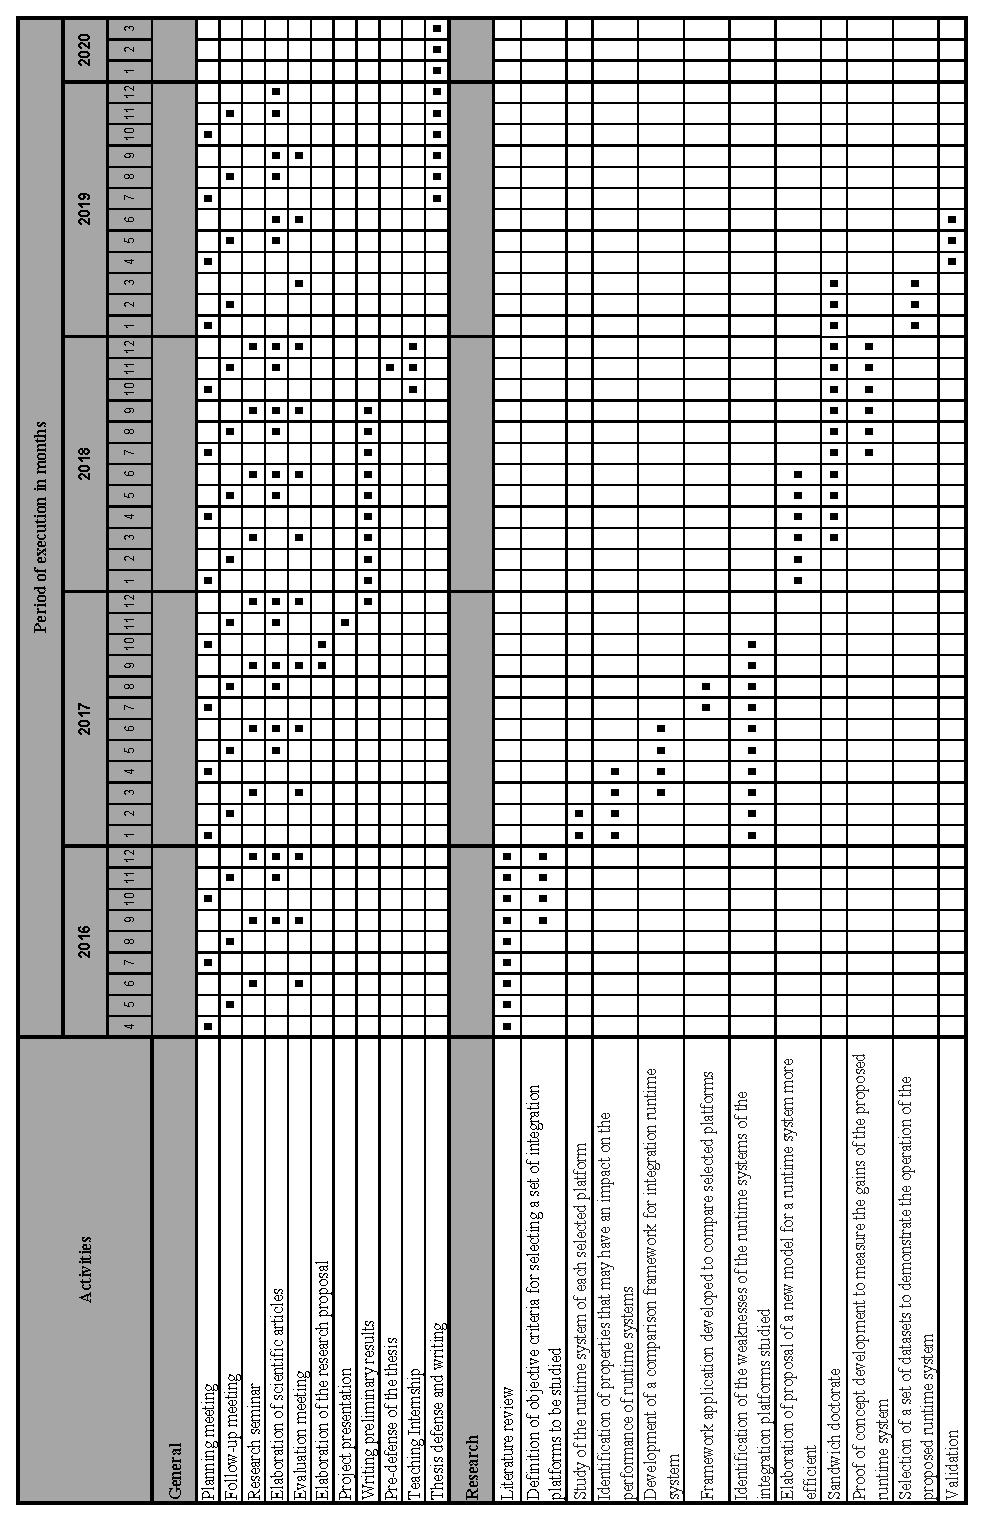
\includegraphics[scale=0.90]{./figs/schedule.eps}
	%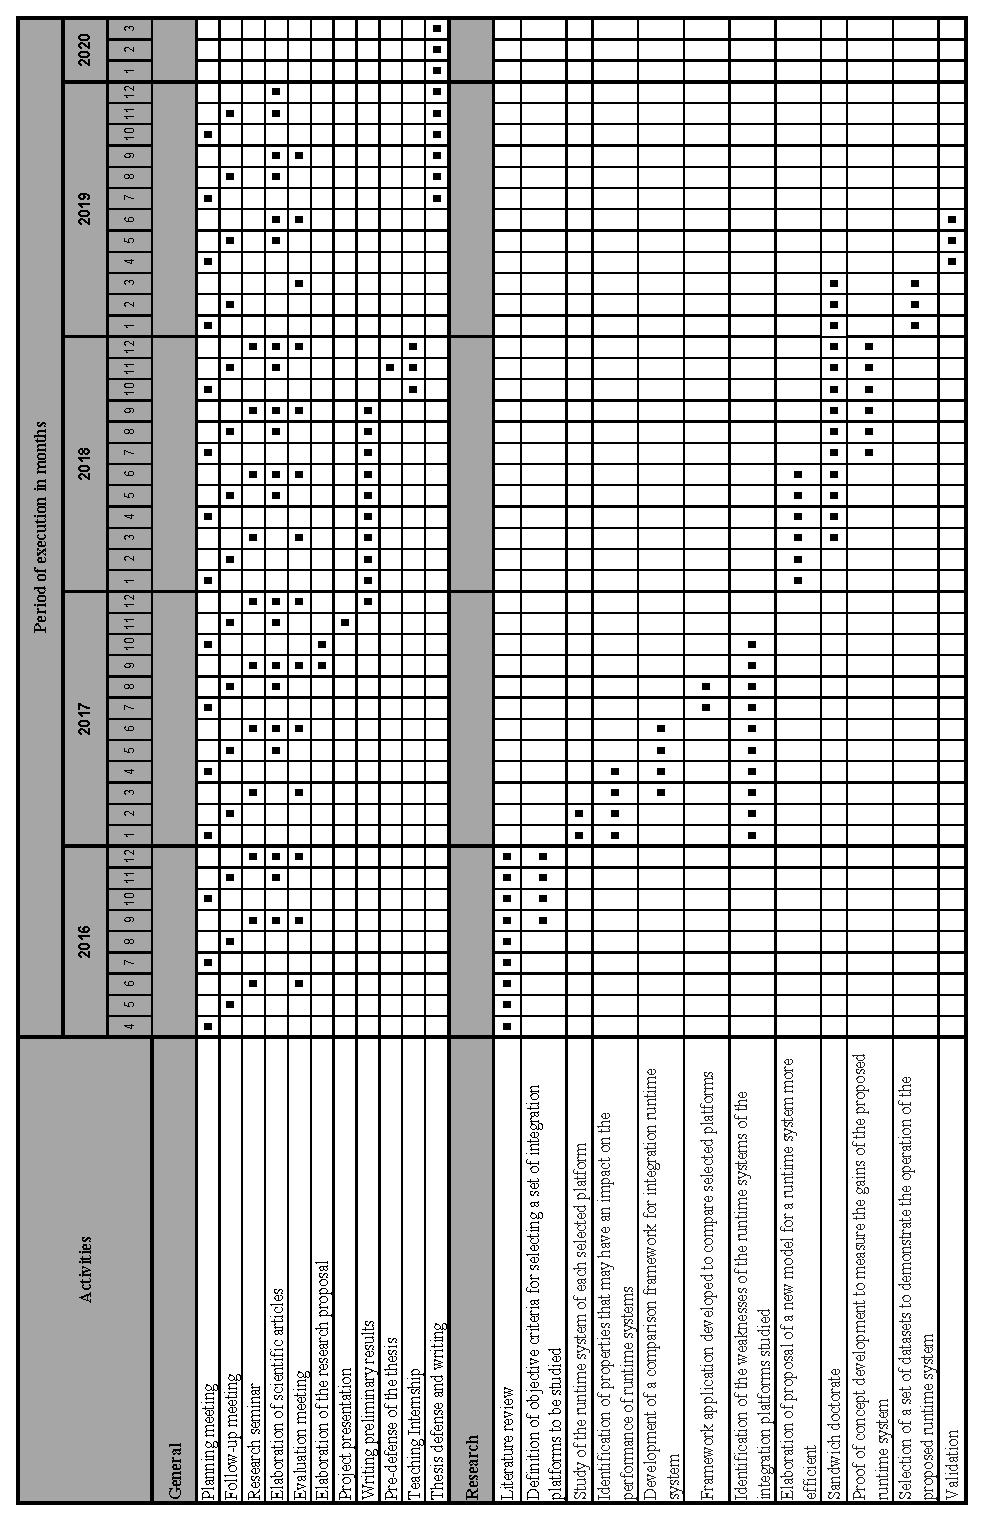
\includegraphics[width=\linewidth]{./figs/schedule.eps}
	\label{tab:schedule1}
\end{table*}

%current stage
In the first year of the research, the research context was studied, including EAI, runtime system, cloud computing and big data. After, a deep literature review was done in order to expand knowledge in the research fields: mathematical modelling, optimization techniques, statistics models and multithread programming. These knowledge form the foundation of our research.
Parallel, criteria for selecting a set of integration platforms to be studied were determined.

From the second year of research, the runtime systems of the selected platforms were studied and properties that may have an impact on their performance were found. With that, a comparison framework for integration runtime systems was developed and applied it in their comparison, and finally, were identified their weaknesses regarding performance. The result generated a partial technical report. During this period, peripheral works were produced, which can lead or contribute to the solutions of the research problems.

The research is currently stating the third step that is the elaboration of a proposal of a new model for a runtime system more efficient.